% Document class report-template accepts either: project-plan or final-report option
\documentclass[project-plan]{report-template}

% Packages I want to use in my report.
\usepackage{graphicx}
\usepackage{amsmath}
\usepackage{blindtext}

% Directory where I save my figures.
\graphicspath{{./figures/}}

% Metadata used for the title page.
\university{Imperial College London}
\department{Department of Earth Science and Engineering}
\course{MSc in Applied Computational Science and Engineering}
\title{Forecasting induced seismicity in Oklahoma}
\author{Zhiyong Liu}
\email{zl1220@ic.ac.uk}
\githubusername{acse-liuzyon}
\supervisors{Dr. Stephen P. Hicks}
\repository{https://github.com/acse-2020/acse2020-acse9-projectplan-liuzyon}

\begin{document}

\maketitlepage  % generate title page
\githubrepo  % GitHub repository

% Abstract
\section*{Abstract}
\blindtext  % outputs some dummy text

% Introduction section
\section{Introduction}
\blindtext[2]

% Another section
\section{My section}
In this work, we implemented code for computing the position of a particle in vertical motion as shown in Fig.~\ref{fig:experiment}. The position $y(t)$ at time $t$ we compute using:

\begin{equation}
    \label{eq:vertical-position}
    y(t) = v_{0}t - \frac{1}{2}gt^{2},
\end{equation}

where $v_{0}$ is the initial velocity, and $g$ is the acceleration due to the Earth's gravity.

\begin{figure}
    \begin{center}
        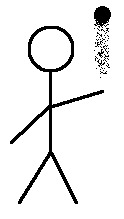
\includegraphics[width=0.2\textwidth]{experiment.jpg}
    \end{center}
    \caption{\label{fig:experiment} Particle in vertical motion.}
\end{figure}

The Python code we implemented for computing $y(t)$ is:

\begin{lstlisting}[language=Python]
def position(t, v0=0, g=9.81):
    """My function."""
    return v0*t - 0.5*g*t**2
\end{lstlisting}

We made our computational workflows reproducible by employing all benefits of the Jupyter environment~\citep{Beg2021}.

\section*{Conclusions}
\blindtext[2]

% References
\bibliographystyle{agsm}
\bibliography{references.bib}  % BibTeX references are saved in references.bib

\end{document}          

